\documentclass[a4paper,twoside,10pt]{book}
\usepackage[margin=3cm]{geometry}
\usepackage[frenchb]{babel}
\usepackage[utf8]{inputenc}
\usepackage{graphicx}
\usepackage{amsmath}
\usepackage{amsmath}
\usepackage{amsfonts}
\usepackage{amssymb}
\usepackage{graphicx}
\usepackage{fancyhdr}
\usepackage{enumitem}
\usepackage{titlesec}
\usepackage[tikz]{bclogo}
\usepackage{pifont}
\frenchbsetup{StandardLists=true}
\usepackage{url}
\usepackage{pdfpages}
\usepackage{eurosym}
\usepackage{lettrine}
\usepackage{wrapfig}
\usepackage{subcaption}
\usepackage{multirow} % pour fusionner des cellules dans un tableau
\usepackage{diagbox} % pour séparer une cellule en diagonale
\usepackage{fontawesome} % pour le symbole haut parleur d'appel de l'enseignant

%%%%%%%%%%%% Pour supprimer les entêtes et pieds de page des pages vierges %%%%%%

\newcommand{\clearemptydoublepage}{%
   \newpage{\pagestyle{empty}\cleardoublepage}}

%%%%%%%%%%%% Définition du titre du chapitre et section %%%%%%%%%%%

\titleformat{\chapter}[frame]{\normalfont}
{\filright \Large \enspace TP n\degre \thechapter\enspace}
{10pt} {\Large\bfseries\filcenter}
\renewcommand{\thesection}{\arabic{section}}

%%%%%%%%%%%% Définition de l'item des questions posées %%%%%%%%%%%

\newlist{question}{enumerate}{2}
\setlist[question,1]{label=\textbf{{Q-\arabic*}:}}
\setlist[question,2]{label=Q-\alph* :}

%%%%%%%%%%%% Entêtes et pied de page %%%%%%%%%%%

\pagestyle{fancyplain}
\renewcommand{\chaptermark}[1]{\markboth{\chaptername\ \thechapter.\ #1}{}}
\renewcommand{\sectionmark}[1]{\markright{\thesection.\ #1}}
\lhead[\fancyplain{}{\bfseries\thepage}]{\fancyplain{}{\bfseries\rightmark}}
\rhead[\fancyplain{}{\bfseries\leftmark}]{\fancyplain{}{\bfseries\thepage}}
\lfoot[\small\slshape Enssat-- Lannion]{\small\slshape TP Optique S4}
\rfoot[\small\slshape 2025--2026]{\small\slshape P. Guillemé}
\rhead[\fancyplain{}{\bfseries\leftmark}]{\fancyplain{}{\bfseries\thepage}}
\cfoot{\fancyplain{\textrm{\thepage}}{}}

%%%%%%%%%%%%% Définition des notations %%%%%%%%%%%

\newcommand{\TF}[1]{\tilde{#1}}
\renewcommand{\u}{u}
\renewcommand{\v}{v}
\newcommand{\f}[1]{\mathfrak{f}_{#1}}


%%%%%%%%%%%%% Commande de notes pour le brouillon du TP
%
%\newcommand{\brouillon}[1]{\texttt{\textcolor{blue}{#1}}}
%
%%%%%%%%%%%%%%%%%%%%%%%%%%%%%%%%%%%%%%%%%%%%%%%%%%%%%%%%%%
\setcounter{tocdepth}{1} 
\begin{document}

\def\figurename{Figure}
\def\tablename{Tableau}

%__________ Définir le chemin des images
%\graphicspath{{TP_OnePix/Images/}}
\graphicspath{{Images/}}


%%%%%%%%%%%%%%% DEBUT DU DOCUMENT %%%%%%%%%%%%%%%%%%%%%%%%%%%%%%%%%%%%%%%%%%%%%%%%%%%%%%%%%%%%%%%%%
\renewcommand{\chaptername}{TP}
\chapter{Optique de Fourier et imagerie monopixel\\
Principe de l'imagerie hyperspectrale}

\vspace{-2\baselineskip}
\begin{center}
\underline{Texte} : Pierre Guillemé
\end{center}

%______________ But du TP
\begin{bclogo}[couleur = gray!10, arrondi = 0.1, logo = \bcinfo, barre = none]{But du TP}
\begin{itemize}
\item Illustrer les notions abordées en cours d'Optique de Fourier pour leur donner un sens concret.
\item Découvrir la technique d'imagerie monopixel.
\item Aborder l’imagerie hyperspectrale.
\end{itemize}
\end{bclogo}

%______________ Compétences
\begin{bclogo}[arrondi = 0.1, logo = \bcquestion]{Compétences à acquérir}
\begin{itemize}[label=\ding{52}]
\item Faire le lien entre l'espace réel et l'espace de Fourier
\item Comprendre un programme Python pour réaliser une transformée de Fourier
\item Utiliser un Notebook Jupyter pour traiter et interpréter des résultats de mesures.
\end{itemize}
\end{bclogo}



%______________ Préparation
\begin{bclogo}[arrondi = 0.1, logo = \bccrayon, barre = none]{Préparation}
Revoir le cours et les TD d'Optique de Fourier et d'imagerie monopixel. Préparer les questions \textbf{Q-1} à \textbf{Q-4} sur votre cahier de manip avant la séance de TP.
\end{bclogo}


%%%%%%%%%%%%%%%%%%%%%%%%%%%%%%%%%%%%%%%%%%%%%%%%%
%
% Introduction
%
%%%%%%%%% 
\section*{Introduction}

Quel est le point commun entre la diffraction, la formation des images à travers une lentille, la limite de résolution d'un appareil optique ou encore l'optique adaptative ?\\
Réponse : toutes s'interprètent de façon rigoureuse à l'aide de l'Optique de Fourier. Son formalisme élégant a permis la compréhension et le développement de nouvelles applications récompensées par des prix Nobel au milieu du XX\up{ème} siècle , telles que l'holographie proposée par Gabor ou encore le microscope à contraste de phase de Zernike.

Si l'analyse de Fourier se révèle redoutablement efficace dans le traitement des problèmes 
d'optique, son formalisme est toutefois rébarbatif et peut poser des difficultés de compréhension. En outre, le développement des calculs fait bien souvent perdre le sens physique des phénomènes mis en jeu. Ce TP est l'occasion de rendre le plus concret possible le lien entre l'espace des images réelles et l'espace de Fourier.

Le début du TP permet d'explorer les fréquences spatiales pour établir un lien intuitif entre celles-ci et les motifs de l'espace réel auxquelles elles sont associées. La suite du TP permet de découvrir une technique d'imagerie particulièrement utile dans le domaine de la biophotonique : l'imagerie hyperspectrale. Enfin, on étudiera l'influence de quelques paramètres physiques du montage sur la qualité des images.




%%%%%%%%%%%%%%%%%%%%%%%%%%%%%%%%%%%%%%%%%%%%%%%%%
%
% Section 1 : 
%
%%%%%%%%%
\section{Préliminaires théoriques}

%________ Subsection_____________________________
\subsection{Rappels mathématiques}

La \emph{transformée de Fourier} (TF) d'une fonction $g$ à deux variables indépendantes $(x, y)$ est définie par :
\begin{equation}\label{eq:defTF}
\TF{g}(\u,\v) = \iint_{-\infty}^{+\infty} g(x, y) \; e^{-2i\pi(\u x + \v y)} dx \; dy
\end{equation}

La fonction $\TF{g}$ obtenue est elle-même une fonction à deux variables $\u$ et $\v$ que l'on appelle les \emph{fréquences spatiales}.

%__________ Boîte à logo remarque
\begin{bclogo}[logo=\bcinfo, noborder=true]{Remarque 1}
En toute rigueur, la transformée de Fourier n'est définie que si :
\begin{itemize}
\item $g$ est absolument intégrable sur $\mathbb{R}^2$,
\item $g$ a un nombre fini de discontinuités et un nombre fini d'extrema dans tout rectangle fini du plan $(x,y)$,
\item $g$ n'a pas de discontinuités infines.
\end{itemize}

Des fonctions couramment utilisées en optique, telle que le \emph{cosinus}, la \emph{distribution de Dirac} $\delta(x,y)$ ou encore la \emph{fonction unité} ne satisfont pas ces conditions d'existence. On définit alors une \emph{transformée de Fourier généralisée}. Pour cela, on peut utiliser une fonction intermédiaire qui satisfait les conditions d'existence de la TF et qui comporte un paramètre que l'on peut faire tendre vers 0 pour retrouver la fonction de départ. Ainsi, la distribution de Dirac peut-elle être vue comme un gaussienne ou une porte infiniment étroite. On peut alors calculer la TF d'une gaussienne de largeur non nulle puis identifier sa limite quand la largeur tend vers 0 à la TF de la distribution de Dirac.

Les TF (ou TF généralisées) des fonctions utiles sont, par exemple, données en annexe A du poly de cours d'Optique Physique de T. Chartier.
\end{bclogo}

La \emph{transformée de Fourier inverse} est définie par :
\begin{equation}\label{eq:TFinverse}
g(x,y) = \iint_{-\infty}^{+\infty} \TF{g}(\u,\v) \; e^{+2i\pi(\u x + \v y)} d\u \; d\v
\end{equation}

Cette expression montre que $g$ peut être interprétée comme une combinaison linéaire de fonctions élémentaires $\f{u,v}(x, y)$ de la forme $\exp[2i\pi(\u x + \v y)]$ chacune associée à une amplitude $\TF{g}(\u,\v)\; d\u \; d\v$.

%__________ Boîte à logo
\begin{bclogo}[logo=\bcinfo, noborder=true]{Remarque 2}
En particulier, puisqu'une image en niveau de gris peut être décrite par une fonction à deux variables $g(x, y)$ alors elle peut s'écrire comme une combinaison linéaire de fonctions élémentaires $\f{\u,\v}(x, y)$ de la forme $\exp[2i\pi(\u x + \v y)]$.

Comme ces fonctions $\f{\u, \v}(x, y)$ et les amplitudes $\TF{g}(\u,\v)$ qui leur sont associées pour reconstruire l'image par combinaison linéaire sont complexes, on ne peut pas \textit{a priori} les représenter en niveaux de gris... mais nous allons voir au cours de ce TP que nous y parviendrons tout de même avec quelques astuces !
\end{bclogo}

%________ Subsection_____________________________
\subsection{Interprétation en terme d'ondes planes}

Après ces quelques rappels mathématiques, venons-en à l'utilisation de ce formalisme en optique. On y a recours dans deux cas :
\begin{itemize}
\item pour écrire une onde monochromatique quelconque sous forme de superposition d'ondes planes,
\item pour décomposer une image en niveaux de gris sous forme d'une superposition de motifs sinusoïdaux élémentaires.
\end{itemize}
Le premier cas est celui étudié en cours d'Optique de Fourier. Puisqu'il vous est familier, nous allons l'utiliser pour acquérir une intuition du lien entre l'espace réel et l'espace de Fourier.

Considérons pour cela une onde lumineuse plane monochromatique de fréquence $\nu$ se propageant sans atténuation selon le vecteur d'onde $\vec{k}$ représenté sur la figure \ref{fig:definitions} (a). L'expression complexe d'une telle onde s'écrit :
\begin{equation}
U(\vec{r}, t) = U_0 \; e^{i(\vec{k}.\vec{r} - 2\pi \nu t + \varphi)}
\end{equation}
où les constantes réelles $U_0$ et $\varphi$ sont respectivement l'amplitude et la phase à l'origine de l'onde. Physiquement $U$ peut-être le champ électrique\footnote{Plus exactement, c'est la partie réelle de $U$ qui représente le champ électrique puisque celui-ci est une grandeur physique réelle.} associé à la lumière éventuellement normalisé pour que sa norme au carré donne directement l'éclairement. On considère ici que la lumière n'est pas polarisée et on se contente donc d'une description scalaire. En regroupant la variation temporelle et la phase à l'origine avec l'amplitude, on définit une amplitude complexe $\underline{U}_0(t)$ qui permet l'expression plus compacte suivante :
\begin{equation}
U(\vec{r}, t) = \underline{U}_0(t) \; e^{i(\vec{k}.\vec{r})}
\end{equation}
En développant le produit scalaire et en utilisant $k = \frac{2\pi}{\lambda}$ on obtient :
\begin{equation}\label{eq:UOndePlane}
U(\vec{r}, t) = \underline{U}_0(t) \; e^{i\frac{2\pi}{\lambda}\gamma z} \; e^{i \frac{2\pi}{\lambda}(\alpha x + \beta y)}
\end{equation}
$(\alpha, \beta, \gamma)$ étant les coordonnées du vecteur unitaire $\hat{k} = \frac{\vec{k}}{k}$. Du fait de la norme unitaire de $\hat{k}$, on a :
\begin{equation}
\gamma = \sqrt{1 - \alpha^2 - \beta^2}
\end{equation}

Si on compare les deux expressions (\ref{eq:TFinverse}) et (\ref{eq:UOndePlane}), on voit qu'une exponentielle complexe $\exp[2i\pi(\u x + \v y)]$ de fréquence spatiale $\u$ et $\v$ peut être interprétée comme une onde plane se propageant dans la direction indiquée par le vecteur unité $\hat{k}$ de coordonnées :
\begin{equation}
\hat{k} = 
\left[
\begin{array}{c}
\alpha = \lambda \u\\
\beta = \lambda \v\\
\gamma
\end{array}
\right]
\end{equation}

Inversement, une onde plane monochromatique de longueur d'onde $\lambda$ et de vecteur d'onde
\begin{equation}
\vec{k} = \frac{2\pi}{\lambda}\left[
\begin{array}{c}
\alpha\\
\beta\\
\gamma
\end{array}
\right]
\end{equation}
est caractérisée par deux fréquences spatiales :
\begin{equation}
\u_0 = \frac{\alpha}{\lambda} \text{ et } \v_0 = \frac{\beta}{\lambda}
\end{equation}

Par exemple, la figure \ref{fig:definitions} représente une onde plane dont le vecteur d'onde $\vec{k}$ fait un angle de 80° avec l'axe vertical $x$ et 75° avec l'axe $y$. Dans la suite, on notera ces angles respectivement $\hat{\alpha}$ et $\hat{\beta}$. On peut calculer les fréquences spatiales associées :
\begin{equation}
\u_0 = \frac{\cos(\hat{\alpha})}{\lambda} \text{ et } \v_0 = \frac{\cos(\hat{\beta})}{\lambda} 
\end{equation}
On peut alors représenter le \emph{spectre de l'onde} dans l'espace des fréquences spatiales (Figure \ref{fig:definitions} (b)).

%__________ Figure double horizontale
\begin{figure}[ht!]
  \centering
  \subfloat[]{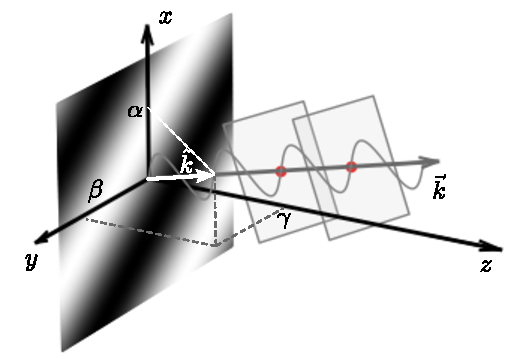
\includegraphics[height=5.5cm]{OndePlane80_75.pdf}}
  \hspace{5pt}
  \subfloat[]{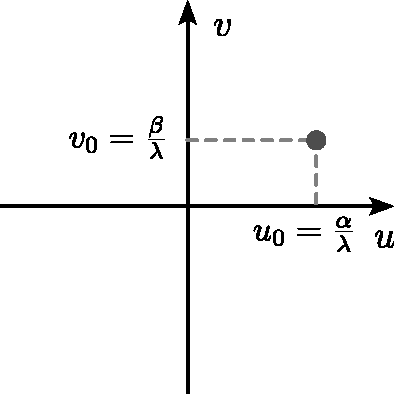
\includegraphics[height=5.5cm]{Spectre_brouillon}}
  \caption{Représentation d'une onde plane (a) et de son spectre (b). Le motif en niveaux de gris représente les valeurs de l'onde $U(x, y, z=0)$ en tout point du plan $z = 0$. Les plans colorés en gris clair sont des plans d'onde espacés d'une longueur d'onde.}
  \label{fig:definitions}
\end{figure}

La figure \ref{fig:definitions} (a) montre aussi un motif en niveaux de gris. Il s'agit de la représentation des valeurs $U(x, y, z = 0)$ prises pas l'onde en chaque point du plan $z = 0$. Les valeurs négatives correspondent aux couleurs sombres. Calculons la distance séparant deux bandes noires successives sur ce motif.
Au niveau de la médiane d'une bande noire, la phase de l'onde est égale à une constante $C_1$ :
\begin{equation}
\frac{2 \pi}{\lambda} (\alpha x + \beta y) = C_1
\end{equation}
L'équation de la droite correspondant à la médiane de cette bande noire est donc :
\begin{equation}
y = - \frac{\alpha}{\beta} x + \frac{C_1 \lambda}{2 \pi \beta}
\end{equation} 
Au niveau de la bande noire voisine, la phase est incrémentée de $2 \pi$. On obtient donc l'équation de droite suivante :
\begin{equation}
y = - \frac{\alpha}{\beta} x + \frac{C_1 \lambda}{2 \pi \beta} + \frac{\lambda}{\beta}
\end{equation}
Les ordonnées à l'origine de ces deux droites sont respectivement $\frac{C_1 \lambda}{2 \pi \beta}$ et $\frac{C_1 \lambda}{2 \pi \beta} + \frac{\lambda}{\beta}$ donc la distance séparant deux bandes noires successives le long de l'axe $y$ est :
\begin{equation}
d_y = \frac{\lambda}{\beta} = \frac{1}{v_0}
\end{equation}

Les abscisses à l'origines de ces deux droites sont quant à elles respectivement $\frac{C_1 \lambda}{2 \pi \alpha}$ et $\frac{C_1 \lambda}{2 \pi \alpha} + \frac{\lambda}{\alpha}$. La distance séparant deux bandes noires successives le long de l'axe $x$ est donc :
\begin{equation}
d_x = \frac{\lambda}{\alpha} = \frac{1}{u_0}
\end{equation}

La figure \ref{fig:interbandes} résume ces résultats. Elle indique également la fréquence spatiale de l'onde
\begin{equation}
F_0 = (u_0^2 + v_0^2)
\end{equation}

%__________ Figure simple
\begin{figure}[htp]
\centering
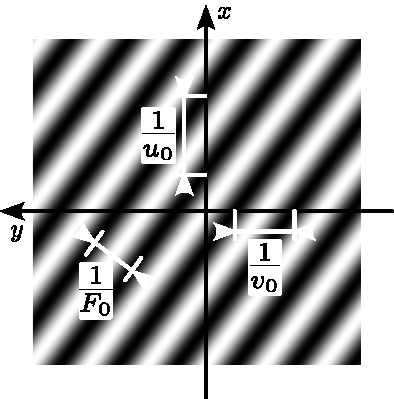
\includegraphics[width=6cm]{Mire_80_75.pdf}
\caption{Représentation du motif sinusoïdal associé à l'onde place de la figure \ref{fig:definitions}.}
\label{fig:interbandes}
\end{figure}

Le calcul précédent montre que les bandes noires sont à l'intersection du plan $(x, y)$ avec les plans d'onde pour lesquels la phase est nulle modulo $2 \pi$. On peut donc intuitivement deviner l'inclinaison et l'espacement des bandes en imaginant comment les plans d'onde (représentés en gris clair sur les figure \ref{fig:definitions} (a)) coupe le plan $(x, y)$.

Nous allons à présent utiliser un Jupyter Notebook pour tracer rapidement des figures telles que la figure \ref{fig:definitions} (a) afin de s'entraîner à faire le lien entre onde plane et spectre de Fourier.

%_____________ Manip
\begin{bclogo}[noborder=true, logo = \bcoutil,barre = line]{Manipulations (\faClockO\ 15 min)}
\begin{itemize}[label=\ding{220}]
\item Télécharger à  partir de Moodle le Jupyter Notebook \texttt{prepa\_tp\_onepix.ipynb}
\item Ouvrir une console (Anaconda powershell prompt sous Windows) et utiliser la commande \texttt{cd adresse\_du\_dossier} pour se placer dans le dossier contenant le Notebook.
\item Taper ensuite \texttt{jupyter lab} pour ouvrir Jupyter Lab.
\item Dans le panneau vertical de gauche, double-cliquer sur le fichier\\ \verb|prepa_tp_onepix.ipynb|. (S'il n'est pas pas présent, on peut l'ajouter en cliquant sur 
\includegraphics[height=5mm]{IconeChargerNotebook}.)
\item Dans le premier script taper \texttt{alpha\_deg = 90} et \texttt{beta\_deg = 80}. Ces variables correspondent à $\hat{\alpha}$ = 90° et $\hat{\beta}$ = 80°.

\item Lancer le premier script en cliquant sur 
\includegraphics[height=5mm]{IconeLancerScript} en haut du Notebook pour valider les valeurs entrées.
\item Le 2\up{ème} script est plutôt long, s'il est affiché, cliquer sur la barre verticale bleue présente dans la marge à gauche pour le replier.
\item Lancer le deuxième script en cliquant sur 
\includegraphics[height=5mm]{IconeLancerScript}.
\item Observer le vecteur d'onde (en orange), les plans d'onde et le motif en niveau de gris dans le plan $z=0$. On peut enregistrer la figure en cliquant sur 
\includegraphics[height=5mm]{IconeDisquette} qui apparaît au survol de la souris sur la figure.
\item Faire varier $\hat{\beta}$ et observer l'évolution des franges du motif sinusoïdal.
\item Fixer ensuite $\hat{\beta}$ = 90° et faire varier $\hat{\alpha}$.
\end{itemize}
\end{bclogo}

\begin{question}
\item Enregistrer quelques figures issues des essais précédents pour illustrer que lorsque le vecteur d'onde est dans le plan horizontal $(y, z)$ alors les franges sont verticales. Que vaut alors la fréquence spatiale $\u_0$ ?
\item Même question quand $\vec{k}$ est dans le plan vertical $(x, z)$.
\item Comment évoluent les franges lorsque le vecteur d'onde se rapproche de l'axe $z$ ?
\end{question}

%________ Subsection_____________________________
\subsection{Spectre de Fourier}

En appliquant la définition de la TF inverse (équation \ref{eq:TFinverse}) à une onde monochromatique quelconque\footnote{Quelconque s'entend par opposition à plane, c'est-à-dire qu'en un plan $z = z_0$ l'amplitude n'est pas constante mais dépend de $x$ et $y$.} se propageant dans la direction $z$, on obtient :
\begin{equation}\label{eq:TFinverseU}
U(x,y, z=z_0) = \iint_{-\infty}^{+\infty} \TF{U}(\u,\v, z = z_0) \; e^{+2i\pi(\u x + \v y)} d\u \; d\v
\end{equation}
C'est-à-dire que l'onde quelconque s'exprime comme une combinaison linéaire d'ondes planes élémentaires ayant chacune comme amplitude la TF de $U$ calculée dans le plan $z = z_0$.

L'ensemble des valeurs $\TF{U}(\u, \v, z = z_0)$ des amplitudes des ondes élémentaires calculées dans le plan $z = z_0$ pour toutes les fréquences spatiales $(\u, \v)$ définissent le \emph{spectre de l'onde} dans le plan $z = z_0$, noté $S_{z_0}(\u, \v)$ et obtenu par TF de $U$ :

\begin{equation}
S_{z_0}(\u, \v) = \iint_{-\infty}^{\infty} U(x, y, z_0) \; e^{-2i\pi (\u x, \v y)} \; dx \; dy
\end{equation}

%________ Subsection_____________________________
\subsection{Application aux images en niveaux de gris - TF discrète}

Venons-en à présent au deuxième cas d'utilisation du formalisme de Fourier en optique.
Comme nous l'avons rapidement évoqué dans le rappel mathématique, une image en niveaux de gris  peut être décrite par une fonction à deux variables $g(x, y)$ et on peut donc utiliser le formalisme de Fourier pour la décrire comme une combinaison linéaire de fonctions sinusoïdales élémentaires\footnote{Et nous n'aurons pas les soucis de rigueur signalés dans la remarque 1 avec les images, si ce n'est le premier point.}.

Etant donné que les images que nous allons utiliser seront des images numériques, donc constituées de pixels plutôt que de variations continues de niveaux de gris, nous allons utiliser la transformée de Fourier discrète. Cela nous permettra en outre de calculer numériquement les TF.

Commençons par revoir la définition de la transformée de Fourier discrète à l'aide du Jupyter Notebook.

%_____________ Manip
\begin{bclogo}[noborder=true, logo = \bcoutil,barre = line]{Manipulations (\faClockO\ 15 min)}
\begin{itemize}[label=\ding{220}]
\item Suivre la partie II du Jupyter Notebook pour programmer \og à la main \fg{} la transformée de Fourier discrète et comparer les résultats obtenus à ceux donnés par le calcul automatique.
\end{itemize}
\end{bclogo}

\begin{question}[resume]
\item Rappeler l'expression de la transformée de Fourier discrète.
\item Reproduire la figure obtenue dans la partie 5) du Jupyter Notebook et commenter. Expliquer entre autre le rôle de la fonction \texttt{fftshift}.
\end{question}



%%%%%%%%%%%%%%%%%%%%%%%%%%%%%%%%%%%%%%%%%%%%%%%%%
%
% Section 2 : 
%
%%%%%%%%%
\section{De la définition mathématique de la TF à son implémentation physique}

L'imagerie monopixel consiste à acquérir non pas directement une image mais son spectre de Fourier puis d'en faire la transformée de Fourier inverse. Comme brièvement évoqué dans la remarque 2 du début de sujet, quelques astuces vont être nécessaires pour obtenir le spectre de Fourier d'une image, c'est l'objet de cette section. La figure \ref{fig:principe} résume le principe qui va être développé dans la suite.

%__________ Figure simple
\begin{figure}[htp]
\centering
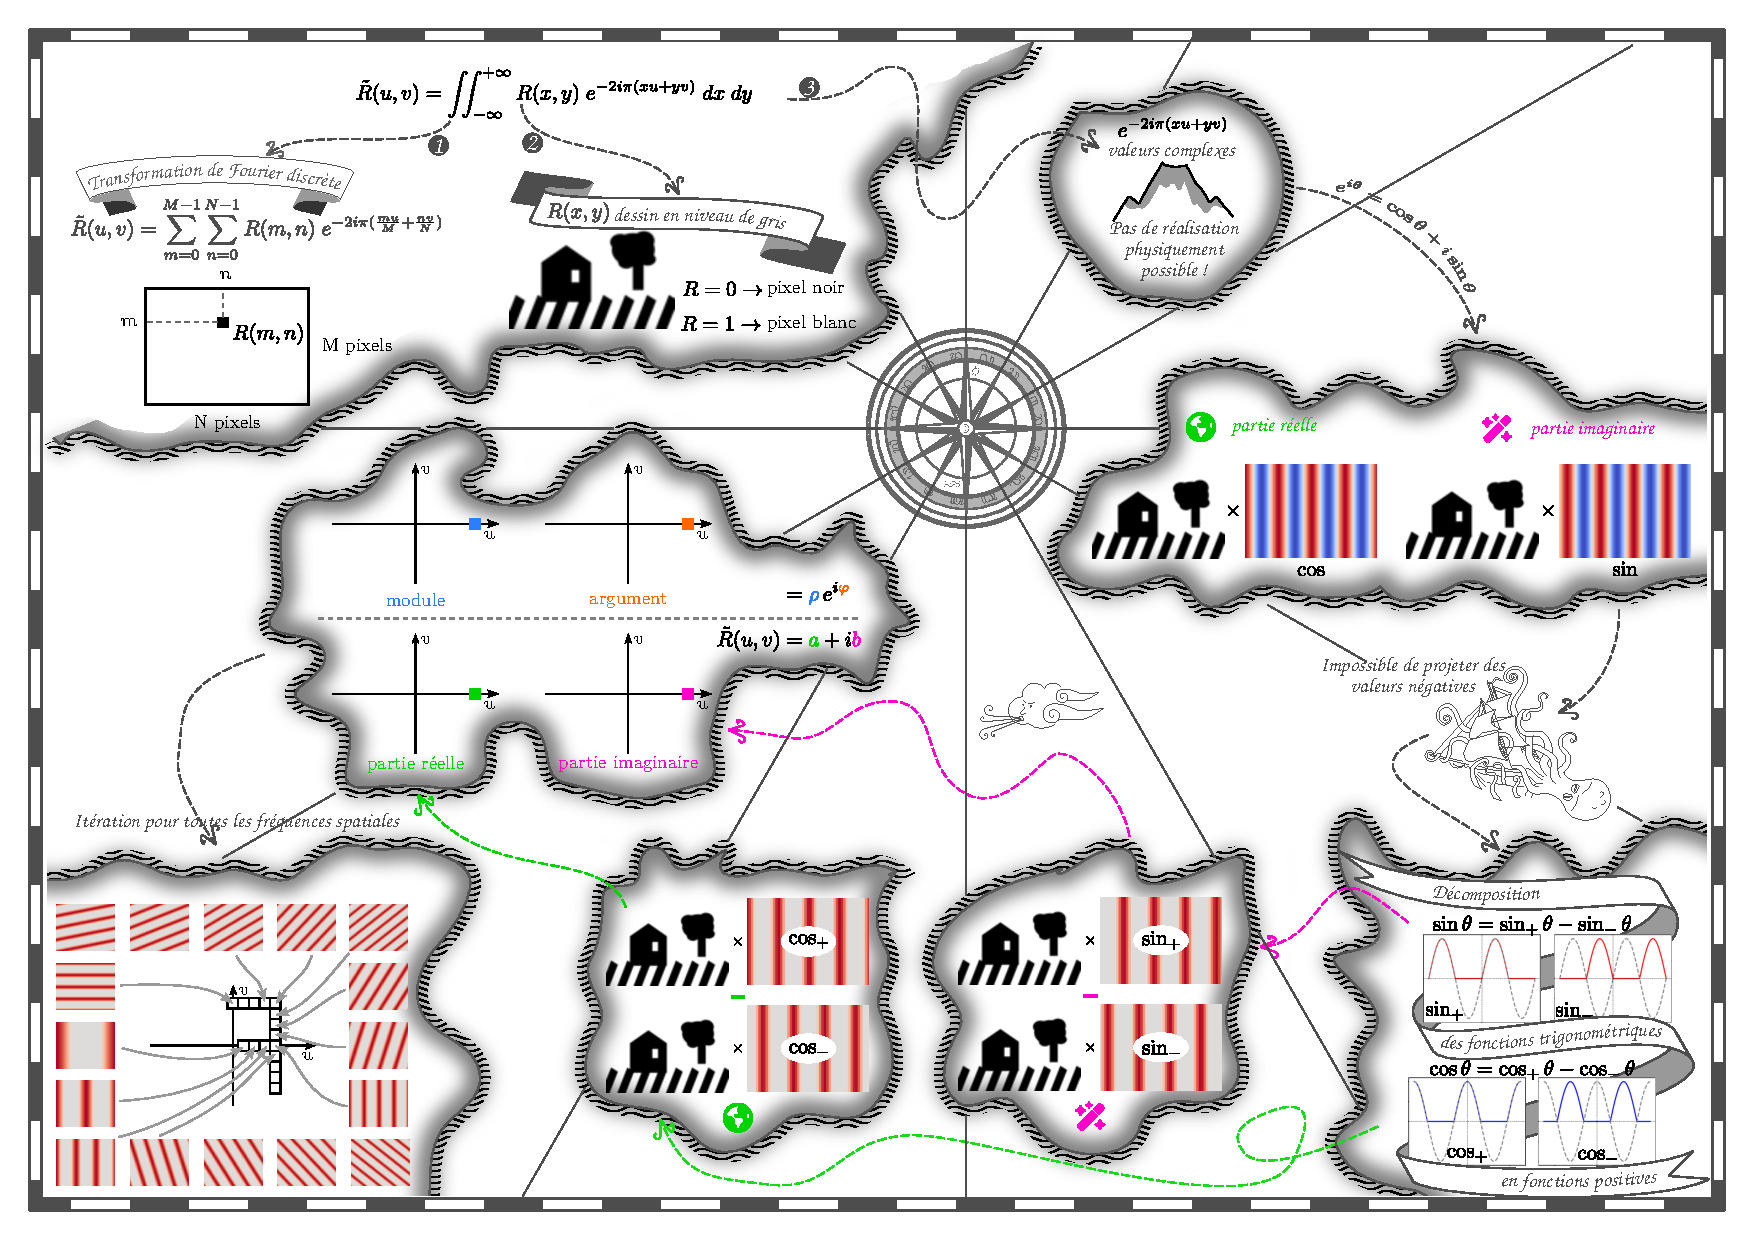
\includegraphics[width=23cm, angle=90]{Carte_One-Piece.pdf}
\caption{Principe de l'imagerie monopixel dans les \og Grand Line \fg{} }
\label{fig:principe}
\end{figure}



%________ Subsection_____________________________
\subsection{Rappels à l'aide de fonctions simples}

%_____________ Manip
\begin{bclogo}[noborder=true, logo = \bcoutil,barre = line]{Manipulations (\faClockO\ 5 min)}
\begin{itemize}[label=\ding{220}]
\item Faire la partie III 1) du Jupyter Notebook pour revoir rapidement le lien entre les fonctions trigonométriques et leur TF.
\end{itemize}
\end{bclogo}

\begin{question}[resume]
\item Reproduire le résultat du calcul de la TF de la fonction sinus 2D à bandes horizontales et commenter. Indiquer notamment comment évolue le spectre de Fourier si les bandes sont plus serrées ou si elles sont verticales.
\end{question}

%________ Subsection_____________________________
\subsection{Adaptation à une image en niveaux de gris}

Jusqu'à présent, nous avons considéré des fonctions pouvant prendre des valeurs négatives. Ces fonctions sont adaptées à la descriptions d'un champ électrique mais pas à celle d'une image. En effet, une image correspond physiquement à un coefficient de transmission dans le cas où la lumière passe à travers une diapositive par exemple, ou un coefficient de réflexion lorsque la lumière éclaire une affiche par exemple. Ces coefficients ne peuvent prendre que des valeurs comprises entre 0 (correspondant aux points noirs de l'image) et 1 (pour les points blancs).

Au cours du TP, nous étudierons des affiches imprimées en niveaux de gris, l'image correspondra donc à une fonction 2D donnant les valeurs du coefficient de réflexion en chacun de ses points, que l'on notera $R(x,y)$.

Voyons comment la TF est modifiée si nous considérons une fonction en cosinus à laquelle on ajoute une constante pour avoir des valeurs positives.

%_____________ Manip
\begin{bclogo}[noborder=true, logo = \bcoutil,barre = line]{Manipulations (\faClockO\ 5 min)}
\begin{itemize}[label=\ding{220}]
\item Faire la partie III 2) du Jupyter Notebook.
\end{itemize}
\end{bclogo}

\begin{question}[resume]
\item Quelle différence y-a-t-il entre la TF d'une fonction cosinus dont la moyenne est nulle et une fonction cosinus à laquelle est ajoutée une constante pour éliminer les valeurs négatives de la fonction ?
\end{question}

%________ Subsection_____________________________
\subsection{Adaptation pour la projection de motifs en niveaux de gris}

Au cours du TP, on utilise un vidéoprojecteur pour projeter des motifs en niveaux de gris sur un écran. Soit $\mathcal{M}(x, y)$ l'éclairement reçu au niveau de l'écran correspondant à l'un des motifs projetés. Chaque point de l'écran diffuse la lumière reçue.

Dans un premier temps, on suppose que la surface de l'écran est un diffuseur lambertien, c'est-à-dire que sa diffusion est isotrope (la \textbf{luminance} émise par chaque point de l'écran est la même dans toutes les directions).

L'affiche (modélisée par son coefficient de réflexion $R(x,y)$) éclairée par un motif (modélisée par l'éclairement $\mathcal{M}(x, y)$) diffuse la lumière en direction d'une fibre optique munie d'une lentille de collection. Le flux énergétique $P$ (en watt) issu de l'ensemble des points de l'écran et reçu au niveau de la lentille de collection dépendra de l'ouverture de la lentille\footnote{En toute rigueur, il faut tenir compte de l'étendu géométrique du détecteur, pour représenter d'éventuels effets de vignettage.}. Sous réserve que celle-ci observe l'écran sous un angle $\theta$ réduit ($\cos \theta$ reste proche de 1 du centre au bord de l'écran), on peut écrire la proportionnalité :
\begin{equation}
P \propto \iint R(x_0, y_0) \times \mathcal{M}(x_0, y_0) \; dx \; dy
\end{equation}

On a vu dans le Jupyter Notebook que la TF discrète de $R(x, y)$ s'écrit :
\begin{equation}
\tilde{R}(u,v) = \sum_{m=0}^{M-1} \sum_{n=0}^{N-1} R(m,n) \; \exp \left[ -2i\pi \left( \frac{mu}{M} + \frac{nv}{N} \right) \right]
\end{equation}

Pour que le flux $P$ corresponde à la double somme permettant de calculer l'élément $\TF{R}(\u_i, \v_j)$ du spectre de Fourier de l'image, il faut que le motif $\mathcal{M}(x, y)$ soit de la forme $\exp[-2i\pi(\u_i x + \v_j y)$.
Il faudrait donc projeter la fonction exponentielle complexe de la forme $\f{\u_i, \v_j}(x, y) = \exp[-2i\pi(\u_i x + \v_j y)]$. Puis en faisant varier $\u$ et $\v$ on mesurerait successivement les amplitudes $\tilde{R}(\u, \v)$ constituant l'ensemble du spectre de l'image.

Projeter une image prenant des valeurs complexes et négatives étant impossible, l'astuce consiste à décomposer l'exponentielle complexe sous la forme :
\begin{align}
\exp[-2i\pi(\u_i x + \v_j y)] & = \cos_+[2\pi(\u_i x + \v_j y)] - \cos_-[2\pi(\u_i x + \v_j y)]\\
& - i(\sin_+[2\pi(\u_i x + \v_j y)] - \sin_-[2\pi(\u_i x + \v_j y)])
\end{align}
où
\begin{equation}
\cos_+(x) = 
\left|
\begin{array}{l}
\cos(x) \text{ quand }\cos(x) \geq 0\\
0 \text{  quand }\cos(x) < 0
\end{array}
\right.
\end{equation}
et
\begin{equation}
\cos_-(x) = 
\left|
\begin{array}{l}
0 \text{ quand }\cos(x) \geq 0\\
-\cos(x) \text{  quand }\cos(x) < 0
\end{array}
\right.
\end{equation}
de même pour $\sin_+$ et $\sin_-$ (Figure \ref{fig:fonctionsTrigo}).

%__________ Figure simple
\begin{figure}[htp]
\centering
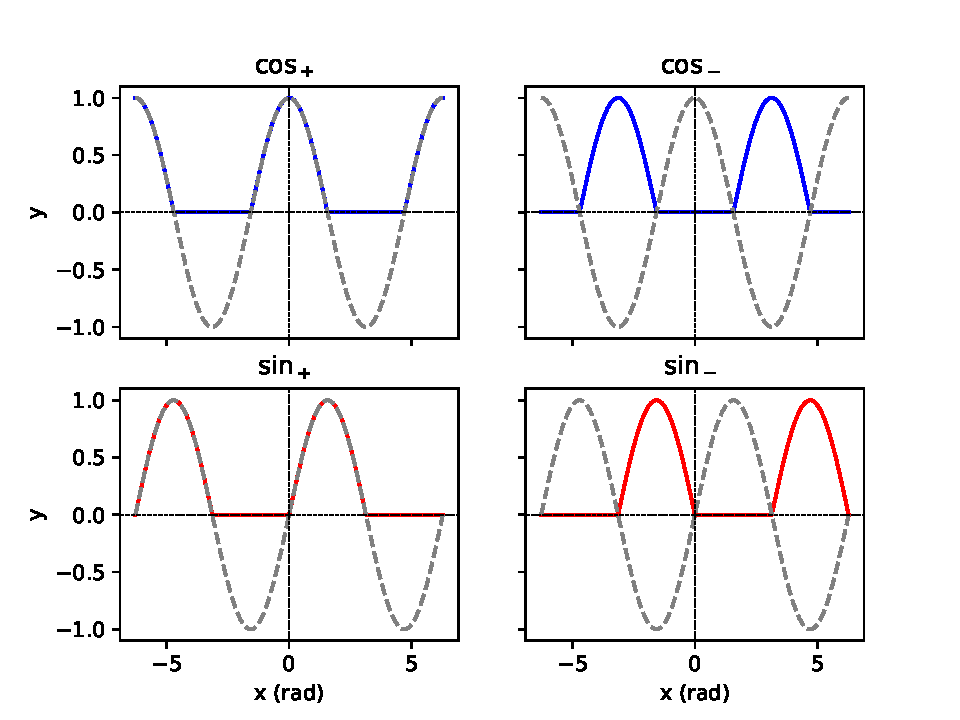
\includegraphics[width=10cm]{FonctionsTrigo.pdf}
\caption{Graphes des fonctions trigonométriques utiles à la projection de motifs en niveaux de gris.}
\label{fig:fonctionsTrigo}
\end{figure}



\begin{question}[resume]
\item Combien de motifs doivent être projetés pour déterminer le terme $\tilde{R}(\u_i, \v_j)$ du spectre de l'image ?
\end{question}

%_____________ Manip
\begin{bclogo}[noborder=true, logo = \bcoutil,barre = line]{Manipulations (\faClockO\ 5 min)}
\begin{itemize}[label=\ding{220}]
\item Faire la partie IV du Jupyter Notebook.
\end{itemize}
\end{bclogo}

\begin{question}[resume]
\item Utiliser le Jupyter Notebook pour illustrer le calcul d'un des pixels du spectre de l'image.
\end{question}

En fin d'acquisition, le logiciel du One-Pix fait une TF inverse du spectre qui a été mesuré pour afficher l'image correspondante.

%_____________ Manip
\begin{bclogo}[noborder=true, logo = \bcoutil,barre = line]{Manipulations (\faClockO\ 5 min)}
\begin{itemize}[label=\ding{220}]
\item Lancer le Jupyter Notebook \texttt{reconstruction.ipynb} pour observer le mécanisme de reconstruction d'une image à partir de son spectre.
\end{itemize}
\end{bclogo}



%%%%%%%%%%%%%%%%%%%%%%%%%%%%%%%%%%%%%%%%%%%%%%%%%
%
% Section 3 : 
%
%%%%%%%%%
\section{Principes de fonctionnement du TP}

L'imageur OnePix se compose principalement d'un Raspberry, un vidéoprojecteur, une fibre munie d'une lentille de collection et d'un spectromètre (Figure \ref{fig:montage}).
Le vidéoprojecteur a été modifié de façon à projeter des images en niveaux de gris. Le Raspberry synchronise la projection de motifs par le vidéoprojecteur avec les acquisitions de spectres\footnote{Il y a beaucoup de spectres dans ce TP 
\includegraphics[height=4mm]{ghost}. Ne pas confondre le spectre fourni par le spectromètre et le spectre de Fourier.} par le spectromètre.

%__________ Figure simple
\begin{figure}[htp]
\centering
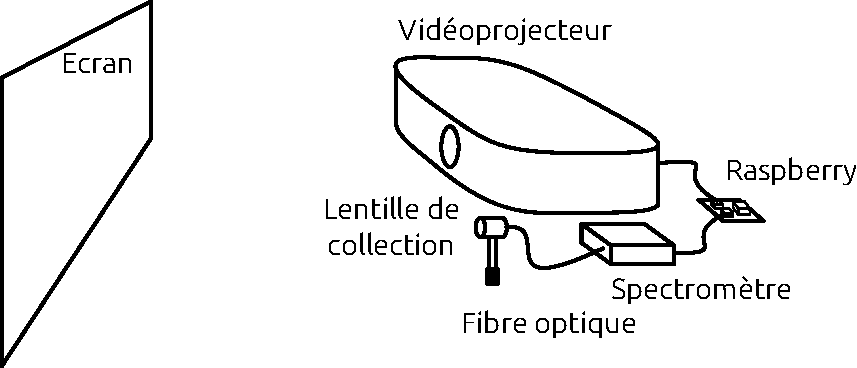
\includegraphics[width=9.5cm]{Montage}
\caption{Schéma du montage constituant l'imageur OnePix.}
\label{fig:montage}
\end{figure}

Pour acquérir une image hyperspectrale, le OnePix projette successivement les motifs correspondant aux fonctions $\cos_+$, $\cos_-$, $\sin_+$ et $\sin_-$ sur la scène à imager et mesure les spectres (en longueurs d'onde) de la lumière diffusée par les objets éclairés. Si la scène contient la fréquence spatiale correspondant au motif projeté, alors la lumière recueillie par le spectromètre est intense. Au contraire, si la fréquence spatiale est absente, le spectromètre recueille peu de lumière diffusée. Faisons une première expérience pour illustrer ce principe élémentaire de fonctionnement.

%_____________ Manip
\begin{bclogo}[noborder=true, logo = \bcoutil,barre = line]{Manipulations (\faClockO\ 20 min)}
\begin{itemize}[label=\ding{220}]
\item Au besoin, glisser l'écran le long du rail pour l'éloigner au maximum du vidéoprojecteur (Distance écran-vidéoprojecteur : $D$ = 82 cm).
\item Brancher le Raspberry et allumer le vidéoprojecteur.
\item Utiliser les aimants pour fixer l'image correspondant aux fréquences spatiales $(\u_0 = 4, \v_0 = 0)$ sur l'écran.
\item Sur le Raspberry pilotant l'expérience, ouvrir un terminal en cliquant sur 
\includegraphics[height=5mm]{Terminal} dans la barre des tâches en haut.
\item Taper \verb|cd Desktop/ONE_PIX_web_socket2| pour se placer dans le dossier contenant l'application qui gère le TP.
\item Taper \verb|python demo_ortho_fonction.py| pour lancer le programme permettant de projeter les motifs voulus et d'acquérir des spectres.
\item Entrer les valeurs de fréquences spatiales voulues $(\u_0 = 4, \v_0 = 0)$ puis cliquer sur \texttt{Valider}.
\item Cliquer sur \texttt{cos+} pour projeter le motif correspondant à $\cos_+(\u_0 x + \v_0 y)$.
\item Cliquer sur \verb|Acquérir spectre| pour acquérir le spectre et afficher la puissance moyenne recueillie, notée $c_+$.\\
Remarque : modifier le temps d'intégration en cas de saturation.
\item Procéder de même avec les motifs suivants. Les puissances correspondantes seront notées $c_-$, $s_+$ et $s_-$.
\item En déduire les valeurs des parties réelle et imaginaire du terme $\tilde{R}(\u_0, \v_0)$ du spectre de Fourier de l'image affichée. 
\item Projeter ensuite les motifs nécessaires à la détermination du terme $\tilde{R}(\u_1 = 2, \v_1 = 0)$ du spectre de Fourier et calculer les valeurs de ses parties réelle et imaginaire.
\end{itemize}
\end{bclogo}

\begin{question}[resume]
\item Comparer les résultats et commenter.
\end{question}


%_____________ Manip
\begin{bclogo}[noborder=true, logo = \bcoutil,barre = line]{Manipulations (\faClockO\ 5 min)}
\begin{itemize}[label=\ding{220}]
\item Fermer les consoles, elles ne seront plus utilisées dans la suite.
\item Cliquer sur l'icône 
\includegraphics[height=10mm]{Icone} pour lancer le logiciel OnePix permettant l'acquisition d'image.
\item Dans la fenêtre de dialogue, cliquer sur \texttt{Exécuter}.
\item Choisir le mode \texttt{Advanced} et cliquer sur \texttt{Complete acquisition}.
\item Dans la fenêtre de dialogue, \textit{Do you want your data to be normalized ?}, cliquer sur \texttt{NO}.
\item Le logiciel ONE-PIX met du temps à se lancer \includegraphics[height=5mm]{Hourglass}
\item Cliquer sur \texttt{Expert}
\item Dans le menu \texttt{Stub}, sélectionner le spectromètre \texttt{Avantes}.
\item Cliquer sur \texttt{Spectrometer connection}.
\item Configurer l'acquisition avec les paramètres suivants :
\begin{itemize}
\item Integration time : 8 ms
\item Image resolution : 21 pixels
\end{itemize}
\item Lancer l'acquisition en cliquant sur \texttt{Acquire hypercube}.
\item Observer l'image réelle et puis cliquer sur \texttt{Image domain <--> Frequency} pour observer le spectre obtenu à l'issue de l'acquisition.
\end{itemize}
\end{bclogo}

\begin{question}[resume]
\item Décrire ce qui se passe pendant l'acquisition et faire le lien avec la préparation théorique. Illustrer notamment le parcours des fréquences dans l'espace de Fourier.
\end{question}


%%%%%%%%%%%%%%%%%%%%%%%%%%%%%%%%%%%%%%%%%%%%%%%%%
%
% Section 4 : 
%
%%%%%%%%%
\section{Exemples d'acquisitions d'images}

%------------------------------------------------
\subsection{Images contenant peu de fréquences spatiales}

%_____________ Manip
\begin{bclogo}[noborder=true, logo = \bcoutil,barre = line]{Manipulations (\faClockO\ 50 min)}
\begin{itemize}[label=\ding{220}]
\item Fixer sur l'écran une affiche au choix présentant une image contenant deux fréquences spatiales.
\item Procéder à l'acquisition via le logiciel One-Pix en cliquant sur \texttt{Acquire hypercube}
\item Utiliser le dispositif et les images à disposition pour retrouver les propriétés connues des TF et répondre aux questions suivantes.
\end{itemize}
\end{bclogo}

\begin{question}[resume]
\item Illustrer le lien entre fréquence spatiale et allure des bandes d'un motif sinusoïdal à bandes verticales.
\item Illustrer le lien entre spectre de Fourier et inclinaison d'un motif sinusoïdal.
\item Montrer l'influence d'une translation de l'image affichée sur le spectre de Fourier.
\end{question}


%------------------------------------------------
\subsection{Exemple d'un dessin simple}

%_____________ Manip
\begin{bclogo}[noborder=true, logo = \bcoutil,barre = line]{Manipulations (\faClockO\ 20 min)}
\begin{itemize}[label=\ding{220}]
\item Afficher l'image de l'arbre et de la maison.
\item Configurer l'acquisition avec les paramètres suivants :
\begin{itemize}
\item Integration time : 8 ms
\item Image resolution : 21 pixels
\end{itemize}
\item Lancer l'acquisition.
\item Faire une nouvelle acquisition en augmentant la résolution à 31 pixels.
\end{itemize}
\end{bclogo}

\begin{question}[resume]
\item Afficher côte à côte les spectres et les images reconstituées. Commenter.
\end{question}



%%%%%%%%%%%%%%%%%%%%%%%%%%%%%%%%%%%%%%%%%%%%%%%%%
%
% Section 5 : 
%
%%%%%%%%%
\section{Principe de l'imagerie hyperspectrale}

Jusqu'à présent, nous avons utilisé le OnePix pour faire des images en niveaux de gris d'une scène. Les images sont longues à acquérir et de mauvaise qualité comparées à ce que donnerait une simple webcam, cependant, nous allons voir que ces images hyperspectrales sont plus riches qu'une simple image.

%_____________ Manip
\begin{bclogo}[noborder=true, logo = \bcoutil,barre = line]{Manipulations (\faClockO\ 20 min)}
On se propose de comparer l'image spectrale d'une feuille fraîche et de sa photocopie couleur.
\begin{itemize}[label=\ding{220}]
\item Faire l'acquisition en proposant les paramètres adéquats (temps d'acquisition et résolution).
\end{itemize}
\end{bclogo}

\begin{question}[resume]
\item Quelles sont les différences observées ? En quoi une image hyperspectrale est-elle plus
riche qu'une simple image prise à la webcam ?
\item Commenter la résolution spectrale et la résolution spatiale de l'image.
\item Calculer la taille de l’hypercube de données.
\end{question}


%%%%%%%%%%%%%%%%%%%%%%%%%%%%%%%%%%%%%%%%%%%%%%%%%
%
% Section 5 : 
%
%%%%%%%%%
\section{Étude de l'influence de quelques paramètres physiques}

%------------------------------------------------
\subsection{Position et orientation de la lentille et de la fibre de collection}

\begin{question}[resume]
\item Mettre en évidence le vignetage. Quelles précautions faut-il prendre pour l'éviter ?
\item Nous avons supposé plus haut que l'écran se comportait en diffuseur lambertien.
Quels seraient les effets néfastes si cette hypothèse n’était pas vérifiée ?
\end{question}

%------------------------------------------------
\subsection{Temps d'intégration}

\begin{question}[resume]
\item Enoncer les critères permettant d’optimiser le temps d’intégration. Modifier et faire
un \verb|acquire spectrum|.
\end{question}

%%%%%%%%%%%%%%%%%%%%%%%%%%%%%%%%%%%%%%%%%%%%%%%%%
%
% Biblio
%
%%%%%%%%%

\vspace{-5mm}

\addcontentsline{toc}{section}{Bibliographie}
\vskip 0.5cm
\begin{bclogo}[noborder=true,logo = \bcbook,barre=none]{\Large Bibliographie}
\vskip 0.25cm
\begin{itemize}[label=\ding{47}]
    \item T. Chartier, \textit{Cours d'Optique Physique}, Enssat, PHOT1
	\item M. Barbier,  \textit{Cours d'Optique de Fourier}, Enssat, PHOT2
	\item Wiki ONE-PIX :\\
	\texttt{https://github.com/PhotonicsOpenProjects/ONE-PIX?tab=readme-ov-file}\\
	Cliquer notamment sur le \texttt{here} situé sous la première image
	\item https://legacy.imagemagick.org/Usage/fourier/
	\item J. Goodman, \textit{Introduction to fourier Opics}, McGraw-Hill, 2nd edition, 1996
	\item H. Ollivier et O. De Melo : \textit{Elementary Fourier Optics for Science and Engineering Students}, IOPScience 2025
\end{itemize}
\end{bclogo}

\end{document}